\PassOptionsToPackage{colorlinks=true,linkcolor=blue,citecolor=blue,urlcolor=blue}{hyperref}
% REQ-FILE: The above line, \PassOptionsToPackage{} must be very first line.

\documentclass[11pt]{article}

% Encoding and font setup for cross-platform reproducibility
\usepackage[utf8]{inputenc}
\usepackage[T1]{fontenc}
\usepackage{lmodern}

% Improve readability for dense theoretical material
\usepackage{setspace}
\onehalfspacing

% Mathematical notation and table formatting for formal semantics
\usepackage{amsmath, amssymb}
\usepackage{booktabs}
\usepackage{bookmark}
\usepackage{graphicx}

% Theorem environments for definitions, lemmas, and formal statements
\usepackage{amsthm}

% plain style is italic body text (for theorems, lemmas, etc.)
\theoremstyle{plain}
\newtheorem{theorem}{Theorem}[section]
\newtheorem{lemma}[theorem]{Lemma}
\newtheorem{proposition}[theorem]{Proposition}
\newtheorem{corollary}[theorem]{Corollary}
\newtheorem{conjecture}[theorem]{Conjecture}

% definition style = upright body text (for definitions, examples)
\theoremstyle{definition}
\newtheorem{definition}[theorem]{Definition}
\newtheorem{example}[theorem]{Example}

% remark style = upright, lighter weight (for remarks, notes)
\theoremstyle{remark}
\newtheorem{remark}[theorem]{Remark}
\newtheorem{note}[theorem]{Note}

% Bibliography management and hyperlink support
\usepackage{url}
\usepackage{hyperref}
\usepackage{natbib}

% Support multiple author affiliations
\usepackage{authblk}

% Improve typographic quality and line breaking
\usepackage{microtype}

% Categorical and commutative diagrams
\usepackage{tikz}
\usepackage{tikz-cd}
\usetikzlibrary{arrows.meta,calc,fit,positioning,shapes.geometric}

% Callout boxes for examples and emphasis
\usepackage{mdframed}
\usepackage[most]{tcolorbox}

% Keywords macro for structured abstract metadata
\providecommand{\keywords}[1]{\textbf{Keywords: } #1}

% Notation for Raw vs Canonical categories in CEP/CEE
\newcommand{\Raw}{\mathsf{Raw}}
\newcommand{\Canon}{\mathsf{Canon}}

% Reusable figure callout box for visual emphasis
\newcommand{\FigureCallout}[2]{%
  \begin{tcolorbox}[
    colback=gray!5,
    colframe=black!40,
    title={#1},
    fonttitle=\bfseries,
    arc=3pt,
    boxrule=0.5pt,
    width=\linewidth,
    enhanced,
    breakable
  ]
  #2
  \end{tcolorbox}
}

% Paragraph spacing prioritizes readability over traditional indentation
\setlength{\parskip}{0.75em}
\setlength{\parindent}{0em}

% Compact list formatting for dense conceptual content
\usepackage{enumitem}
\setlist[itemize]{itemsep=0.2em, topsep=0.2em, parsep=0em, partopsep=0em}

% Defensive re-definition ensures commands exist if loaded earlier
\providecommand{\Raw}{\mathrm{Raw}}
\providecommand{\Canon}{\mathrm{Canon}}

\title{A Categorical Ontology for Civic Accountable Entities (CAE)}

\author[1,2]{Denise M. Case}
\affil[1]{Northwest Missouri State University, Computer Science and Information Systems, Maryville, MO, USA}
\affil[2]{Civic Interconnect, Ely, MN, USA}

\date{\today}

\begin{document}

\maketitle
\vspace{-1em}

% Explicitly mark preprint status
\begin{tcolorbox}[colback=gray!10, colframe=black!20, boxrule=0.3pt]
  \textbf{Preprint Notice.}
  This preprint has not undergone peer review.
  It is shared to support community discussion, transparency research, and early technical evaluation.
\end{tcolorbox}

\begin{abstract}
  We present a categorical ontology of civic accountable entities (CAE)
  intended as a foundational object universe for formal semantics of civic data systems.
  CAE defines a strict, disjoint partition of entities according to their role in
  exchanges, obligations, authority, and accountability, rather than
  domain, sector, or function.
  The ontology distinguishes six entity kinds:
  Actors, Assets, Instruments, Events, Jurisdictions, and Observations.
  These categories are designed to be invariant under representation,
  stable over time, and sufficient to model long-term public investments,
  regulatory regimes, financial flows, and outcome measurements across
  domains such as procurement, health, environment, education, and infrastructure.

  The ontology is explicitly exchange-driven:
  entities are introduced only insofar as they participate in
  obligations, authority relationships, or accountability-bearing events.
  Roles, classifications, and sectoral labels are modeled as relations
  or attributes rather than entity kinds, ensuring disjointness and
  preventing ontological overlap.
  Laws and regulations are treated as normative and regulatory instruments
  that ground concrete events and outcomes without requiring exhaustive legal modeling.

  CAE is intended to serve as the object-level foundation for
  subsequent category semantics of the Civic Exchange Protocol (CEP)
  and Contextual Evidence and Explanations (CEE).
  By separating ontological commitment from exchange semantics and
  evidentiary reasoning, CAE enables interoperable, auditable, and
  longitudinal analysis of public systems while remaining neutral
  with respect to policy positions or causal claims.
  This structure supports comparative analysis across jurisdictions and time,
  making long-term public outcomes inspectable without
  collapsing into advocacy or narrative-driven interpretation.
\end{abstract}

\begin{keywords}
  Categorical ontology,
  accountable entities,
  civic data,
  public accountability,
  exchange semantics,
  longitudinal outcomes,
  formal semantics.
\end{keywords}

% !TeX root = 00P1_cae_ontology.tex

\section{Introduction and Motivation}
\label{sec:introduction}

Civic systems are governed by complex interactions among laws, institutions,
infrastructure, financial flows, and measured outcomes.
Data describing these systems is typically fragmented across domains such as procurement, public
health, environmental regulation, education, and infrastructure.
While each domain is often supported by mature data systems, the structural relationships
that connect authority, obligation, action, and long-term outcomes are
rarely represented in a unified or
interoperable form~\cite{bowker2000sorting,edwards2011infrastructure}.

This fragmentation presents a fundamental obstacle to accountability and
longitudinal analysis.
Short-term metrics are frequently privileged over
long-term public value, and outcomes that accrue over decades—such as population
health, infrastructure resilience, or environmental quality—are difficult to
relate back to the legal, institutional, and financial decisions that shape
them~\cite{edwards2011infrastructure,kahn2002information}.
As a result, public investments with high upfront costs and diffuse
benefits are systematically undervalued, even when their historical impact is
well established.

Many existing approaches focus either on transactional data (such as payments
or contracts), legal texts (such as statutes and regulations), or outcome
measures (such as health or economic indicators).
Few provide a principled way to connect these elements without
collapsing distinct concepts into a single
layer or embedding interpretive assumptions directly into data models~\cite{bowker2000sorting}.

This paper introduces the Civic Accountable Entities (CAE) ontology as a
foundational response to this challenge.
CAE defines a formal ontology of entities that participate in
obligations, authority, and accountability within civic systems.
Rather than modeling domains or sectors directly, CAE identifies
a small set of disjoint entity kinds that are stable across time and context and
sufficient to represent the structural relationships underlying civic accountability.

The design of CAE emphasizes ontological clarity over descriptive completeness.
Entities are partitioned into disjoint kinds with explicit identity criteria;
roles, classifications, and sectoral labels are modeled as attributes or
relationships rather than as entity kinds.
This discipline prevents ontological overlap and supports formal reasoning
about obligations, authority, and evidence.

CAE draws on foundational work in formal ontology, particularly the
emphasis on rigorous categorization found in BFO~\cite{smith2015bfo} and
DOLCE~\cite{masolo2004wonderweb}, while making commitments tailored to
civic accountability: entities are included in CAE only insofar as they
participate in accountability-bearing relationships, and the ontology
is designed to remain stable as domains, policies, and tooling evolve.
Section~\ref{sec:related} discusses these relationships in detail.

CAE provides the ontological foundation for the Civic Exchange Protocol (CEP),
which models how entities exchange value and authority, and for Contextual
Evidence and Explanations (CEE), which attaches structured explanations to
civic decisions.
By separating what exists from how it moves and how decisions are explained,
CAE enables interoperable, auditable, and longitudinal analysis of public
systems while remaining neutral with respect to policy positions or causal claims.

The remainder of this paper is organized as follows:
Section~\ref{sec:related} situates CAE within related work in formal ontology;
Section~\ref{sec:principles} outlines the design principles and scope
of CAE;
Section~\ref{sec:ontology} defines the six disjoint entity kinds;
Section~\ref{sec:relationships} discusses relationships and structural constraints;
Section~\ref{sec:evaluation} evaluates CAE via competency questions;
Section~\ref{sec:laws} discusses laws, regulations, and accountability chains;
Section~\ref{sec:outcomes} discusses outcomes, observations, and public value;
Section~\ref{sec:discussion} includes discussion and future work;
and Section~\ref{sec:conclusion} provides a conclusion.
       % Introduction and Motivation
% !TeX root = 00P1_cae_ontology.tex


\section{Design Principles and Scope}
\label{sec:principles}

The design of CAE is guided by a small number of explicit principles intended to
ensure clarity, stability, and extensibility.

\subsection{Accountability-Driven Inclusion}

CAE models entities only insofar as they participate in accountability-bearing
relationships.
An entity is introduced when it bears obligations, exercises
authority, participates in regulated actions, or is the subject of measurement
and evaluation.
CAE does not attempt to enumerate all organizations, facilities,
laws, or social phenomena exhaustively.

This exchange and obligation-driven inclusion rule prevents ontological bloat
and ensures that the ontology remains focused on structures that matter for civic
accountability~\cite{bowker2000sorting}.

In CEP, admissibility is determined by the presence of instrument-grounded events involving accountable actors.

\subsection{Disjoint Entity Kinds}

CAE defines a strict partition of entities into disjoint kinds.
Each entity is assigned exactly one kind, and entity kinds do not overlap.
This disjointness is
a foundational constraint: it prevents ambiguity and supports formal reasoning
over relationships.

Changes in function, responsibility, or context are represented through
relationships rather than reclassification.
An entity does not change kind over
time, even as its role within civic systems evolves.

\subsection{Roles as Relationships}

CAE does not model roles, sectors, or functions as entity kinds.
Concepts such as regulator, funder, operator, recipient, or subject of regulation are represented
as patterns of relationships among entities.
This approach avoids proliferation of role-specific entity types and
ensures that entity identity remains stable across contexts.

\subsection{Selective and Lazy Modeling}

Entities, particularly laws and regulations, are included selectively based on
their operational relevance.
Normative or regulatory instruments are introduced
only when they ground concrete events or observations.
This lazy modeling strategy supports scalable implementation
and avoids premature commitment to comprehensive legal or administrative catalogs.

\subsection{Neutrality and Separation of Concerns}

CAE is intentionally neutral with respect to causal inference, evaluative
judgment, and policy interpretation.
The ontology encodes structural
relationships that make accountability and outcomes inspectable,
but it does not assert that particular instruments cause particular
outcomes or that specific outcomes are desirable~\cite{pearl2009causality}.

Interpretation, explanation, and evidentiary reasoning are deferred to analytic
layers built upon CAE, including CEP and CEE.
This separation of concerns
supports transparency, reproducibility, and pluralistic analysis.

\subsection{Durability and Extensibility}

CAE is designed to remain stable over long time horizons.
The entity kinds and structural constraints are intended to be invariant even as institutions,
measurement practices, and data sources evolve~\cite{edwards2011infrastructure}.
Extension occurs through the addition of entities and relationships,
not through modification of the underlying ontology.

This design supports incremental adoption and cross-domain interoperability
without requiring coordinated changes across systems.  % Design Principles and Scope
% !TeX root = 00P1_cae_ontology.tex

\section{Ontological Partition of Accountable Entities}
\label{sec:ontology}

This section defines the core ontological commitment of the Civic Accountable
Entities (CAE) framework.
CAE introduces a strict partition of accountable entities into six disjoint kinds:
Actors (A), Sites/Assets (S), Instruments (I),
Events (E), Jurisdictions (J), and Observations (O).
Each entity instantiated within CAE is assigned exactly one kind.
Entity kinds are invariant over time:
entities do not change kind, and apparent role changes are represented through
relationships rather than reclassification.

The partition is designed to support formal semantics of exchange, authority,
and evidence while preventing ontological overlap.
Inclusion of an entity in CAE is driven by participation in obligations, authority relationships, or
accountability-bearing exchanges, rather than by descriptive completeness or
sectoral classification.

\subsection{Actors (A)}
\label{subsec:actors}

Actors are entities capable of bearing rights, obligations, or responsibilities
within civic systems.
An Actor may initiate, receive, authorize, or be held
accountable for actions governed by Instruments and manifested through Events.
Actors are the only entity kind that may serve as parties to obligations.

Examples of Actors include governments, public agencies, private businesses,
nonprofit organizations, universities, research institutes, and think tanks.
Public or private status, sector, mission, and organizational role are treated
as attributes or relationships, not as entity kinds.

An Actor is introduced into CAE only when it participates in an accountability
relationship, such as receiving funds, issuing authority, operating regulated
Sites, or being subject to reporting or enforcement.
CAE does not attempt to enumerate organizations exhaustively;
rather, it models Actors insofar as they
are implicated in civic exchanges or obligations.

\subsection{Sites and Assets (S)}
\label{subsec:sites}

Sites and Assets are physical or operational entities that are acted upon but do
not themselves bear obligations.
They provide the spatial, infrastructural, or
material substrate upon which civic activity occurs.
Sites and Assets may be owned, operated, regulated, inspected, or measured,
but they are not parties to Instruments.

Examples include facilities, buildings, campuses, power plants, laboratories,
stores, transportation infrastructure, and other physical installations.
Geographic location is an intrinsic property of Sites and Assets and provides a
natural point of attachment to Jurisdictions.

Treating Sites and Assets as a distinct entity kind ensures a clear separation
between accountable actors and the physical or operational entities through
which obligations are exercised or impacts are realized.

\subsection{Instruments (I)}
\label{subsec:instruments}

Instruments are enduring constructs that create, modify, delegate, or constrain
rights, obligations, or authority.
Instruments mediate relationships between Actors and govern the conditions under which Events may occur.
Instruments are not time-indexed occurrences but persistent normative or programmatic entities.

CAE distinguishes conceptual subclasses of Instruments without introducing
additional entity kinds.
These include normative instruments (such as statutes
and laws), regulatory instruments (such as rules and regulations), and
programmatic instruments (such as contracts, grants, permits, licenses, and
formal programs).
All such instruments share the defining property of grounding accountability relationships.

Instruments are included in CAE only when they give rise to concrete Events or Observations.
This design avoids exhaustive modeling of legal or administrative
texts while preserving the causal and accountability structure necessary for
exchange and evidence semantics.

\subsection{Events (E)}
\label{subsec:events}

Events are time-indexed occurrences asserted under the authority of Instruments.
An Event records that something happened at a particular time and place and may
involve one or more Actors, Sites, or Jurisdictions.
Events constitute the primary evidence of activity within civic systems.

Examples include payments, inspections, filings, emissions submissions,
violations, audits, and enforcement actions.
Events are not enduring objects;
their identity is inseparable from their temporal occurrence and provenance.

By separating Events from Instruments, CAE distinguishes between the existence
of obligations and their execution or violation.
This separation is essential for representing compliance, performance, and accountability over time.

\subsection{Jurisdictions (J)}
\label{subsec:jurisdictions}

Jurisdictions are entities that scope authority, applicability, and governance.
They define where Instruments apply, where Events may occur, and where Observations are interpreted.
Jurisdictions are not Actors; they do not initiate actions or bear obligations,
but they structure accountability relationships.

Examples include nations, states, provinces, municipalities, regulatory regions,
air basins, and watersheds.
Jurisdictions may be nested or overlapping, and such
structure is represented explicitly through relationships.

Treating Jurisdictions as a distinct entity kind allows CAE to model legal,
regulatory, and environmental scope without conflating authority with agency or
action.

\subsection{Observations (O)}
\label{subsec:observations}

Observations are measurements or indicators describing the state, performance,
or outcomes associated with Actors, Sites, Instruments, Events, or Jurisdictions.
Observations do not create obligations and do not represent actions; they assert
measured or derived facts with associated provenance.

Examples include health outcomes, coverage rates, emissions intensity, food
access indicators, educational attainment measures, and other longitudinal or
comparative metrics.
Observations may be aggregated, statistical, or model-based
and are typically associated with populations or regions through attributes and
relationships.

Introducing Observations as a first-class entity kind enables CAE to represent
long-term public value, outcomes, and impacts without collapsing measurement into
events or instruments.
This separation supports comparative analysis across time
and jurisdictions while remaining neutral with respect to causal interpretation.         % Ontological Partition of Accountable Entities
\input{04_constraints} % Relationships and Structural Constraints
% !TeX root = 00P1_cae_ontology.tex

\section{Laws, Regulations, and Accountability Chains}
\label{sec:laws}

This section describes how laws and regulations are represented within the CAE
ontology and how they participate in accountability chains without requiring
exhaustive modeling of legal texts.
CAE treats statutes and regulations as Instruments that ground 
authority, obligations, and enforcement while remaining
structurally compatible with exchange and evidence semantics.

The objective is not to encode legal doctrine, but to preserve the causal and
accountability structure through which public authority produces concrete
actions and observable outcomes.

\subsection{Normative and Regulatory Instruments}
\label{subsec:normative}

Within CAE, laws and regulations are modeled uniformly as Instruments.
A statute, act, or treaty is treated as a normative instrument: an enduring
construct that establishes authority, delegates power, or defines obligations at
a high level.
Regulations, rules, and administrative codes are treated as
regulatory instruments: instruments that operationalize normative instruments by
specifying procedures, thresholds, or reporting requirements.

Both normative and regulatory instruments share the defining property of
grounding accountability relationships.
They differ only in scope and level of abstraction, not in ontological kind.
This approach avoids proliferating entity types while preserving 
the hierarchical structure of legal authority.

\subsection{Delegation and Implementation Chains}
\label{subsec:delegation}

Accountability chains emerge through explicit relationships between instruments
and actors.
A normative instrument may delegate authority to one or more Actors,
which in turn issue regulatory or programmatic instruments.
These downstream instruments constrain Events and give rise to Observations.

For example, a statute enacted by a legislature delegates authority to an agency.
The agency issues regulations implementing the statute, which authorize permits
governing the operation of facilities.
Compliance reports, inspections, and violations occur as Events under these permits, 
and population-level impacts are captured as Observations.

Representing delegation and implementation explicitly allows CAE to trace how
authority flows from abstract law to concrete outcomes without conflating
normative intent with execution.

\subsection{Selective Inclusion and Lazy Modeling}
\label{subsec:selective}

CAE does not require comprehensive inclusion of all laws or regulations.
Normative and regulatory instruments are introduced only when they ground
accountability-bearing Events or Observations.
This selective inclusion strategy prevents ontological bloat and supports scalable implementation.

For instance, a health statute need not be modeled until insurance programs,
payments, enforcement actions, or outcome measurements associated with that
statute are introduced.
The presence of an instrument in CAE is therefore driven
by its operational relevance rather than by its legal prominence.

This design ensures that CAE remains extensible and performant while preserving
the structural relationships necessary for downstream semantics.

\subsection{Jurisdictional Scope and Applicability}
\label{subsec:scope}

Every normative or regulatory instrument applies within one or more
Jurisdictions.
Jurisdictional scope is represented explicitly through
relationships rather than being implied by instrument identity.
This allows instruments with overlapping or nested applicability to coexist without ambiguity.

Explicit jurisdictional modeling supports comparative analysis across regions and
time, enabling the study of how differing legal regimes relate to variations in
events and observations.
It also permits instruments to evolve or be superseded
without altering the identity of affected entities.

\subsection{Accountability Chains and Observability}
\label{subsec:chains}

An accountability chain is defined as a connected subgraph linking normative or
regulatory instruments to concrete events and observations through delegation,
issuance, participation, and measurement relationships.
Such chains make explicit how public authority is exercised and how its consequences are observed.

CAE does not assert causal claims within these chains.
Instead, it provides a structural representation that allows causal hypotheses to be articulated,
tested, or debated using evidence attached through CEE.
This separation of structure from inference ensures neutrality while enabling rigorous analysis.

\subsection{Implications for Longitudinal Analysis}
\label{subsec:longitudinal}

By modeling laws and regulations as enduring instruments within accountability
chains, CAE supports longitudinal analysis of public interventions.
Changes in legal regimes, regulatory thresholds, or enforcement practices can be represented
as modifications or additions to instruments and relationships rather than as
redefinitions of entities.

This approach enables comparative study of long-term public investments and
policy choices, such as infrastructure development, public health interventions,
or environmental regulation, while preserving continuity of entity identity
across time.      % Laws, Regulations, and Accountability Chains
\input{06_value}       % Outcomes, Observations, and Public Value
% !TeX root = 00P1_cae_ontology.tex

\section{Relationship to CEP and CEE}
\label{sec:relationship}

The Civic Accountable Entities (CAE) ontology is intended to serve as the
foundational object universe for subsequent categorical semantics of the Civic
Exchange Protocol (CEP) and Contextual Evidence and Explanations (CEE).
CAE defines what kinds of entities exist and how they may be related, while CEP and
CEE define how exchanges and evidence are interpreted over those entities.

CEP operates over CAE entities by assigning formal semantics to patterns of
relationships involving Actors, Instruments, Events, and Sites.
Exchanges, obligations, transfers, and authorizations are expressed as structured
compositions of CAE relationships rather than as new ontological constructs.
Because entity kinds and relationship constraints are fixed at the CAE level,
CEP semantics remain uniform across domains and jurisdictions.

CEE builds upon both CAE and CEP by attaching evidence, provenance, and
explanatory structure to Events and Observations grounded in CAE entities.
Explanatory claims and causal hypotheses are expressed relative to the
accountability chains defined by CAE and the exchange semantics defined by CEP.
This separation ensures that evidence and explanation do not require modification
of the underlying ontology.

Together, CAE, CEP, and CEE form a layered framework in which ontological
commitment, exchange semantics, and evidentiary reasoning are clearly separated
yet composable.
         % Relationship to CEP and CEE
% !TeX root = 00P2_cep_semantics.tex


\section{Limitations and Future Work}
\label{sec:limitations}

The categorical core presented in this paper captures identity,
canonicalization, provenance, and interoperability for discrete,
revision-based civic records.
Several important extensions remain outside the present scope.

Many civic systems also generate data that is statistical, uncertain, or
continuously updated (e.g., longitudinal indicators, evolving aggregates).
Incorporating such information may require probabilistic semantics or
temporal indexing, which are not modeled in the current framework.

Jurisdictions evolve data models over time.
Although CEP supports adapters for structural variation,
a full account of schema evolution, including additions,
deprecations, and long-term migration paths, remains future work.

\paragraph{Multi-Stage and Nested Exchanges.}

Some workflows involve layered or multi-party processes
(e.g., multi-level budget allocations, nested reporting pipelines).
These may benefit from higher-structured categorical tools,
but such extensions lie beyond the scope of this foundational treatment.

\paragraph{Rule Sensitivity in Canonicalization.}

Certain linguistic cases (such as expansions of abbreviations like “S.A.”)
require stratified rule ordering within the normalization pipeline rather
than treating all rewrite rules as freely permutable.
This refinement does not affect the well-definedness of the canonicalization
function but does highlight the need for continued empirical tuning of rule strata.

\medskip

The present semantics establish a robust core for identity and interoperability.
Extending CEP to the richer data practices found across governments and civic ecosystems
is a key direction for future work.

% ------------------------------------------------------------
\section{Conclusion}
\label{sec:conclusion}

We presented a categorical semantics for the Civic Exchange Protocol
that unifies canonicalization, provenance, adapters, and context tags
into a coherent mathematical framework.
This perspective makes explicit the invariants that govern identity,
record evolution, and interoperability across heterogeneous civic data systems.

Canonicalization was formulated as a deterministic monoidal functor,
ensuring stable identifiers and well-defined equivalence classes.
Jurisdictional adapters were modeled as oplax functors, capturing how
local structure may be weakened while preserving global identity.
Context tags were expressed via a fibered category, isolating
interpretive annotations from canonical record content.
Together, these structures yield formal guarantees for identifier preservation,
compositional provenance, and cross-jurisdiction reconciliation.

The resulting semantics provides a rigorous foundation for validation,
verification, and future extensions of CEP.
It enables principled design of domain schemas, vocabularies,
and interoperability standards, while remaining extensible to evolving civic workflows.
As civic data ecosystems continue to grow in scale and complexity,
categorical methods offer a durable and expressive language for ensuring that shared
identities and exchanges remain consistent, transparent, and reliable.


\section*{Acknowledgements}

Portions of this work were developed through human-computer collaboration
using modern computational tools.
Generative language models were used to assist with editing, formatting,
and consistency checking during manuscript preparation.
All conceptual framing, formal development, results, interpretations, and conclusions
are the author's own.
All generated suggestions were critically reviewed and validated, and
the author takes full responsibility for the content of this work.  % Limitations, Future Work, Conclusion

\appendix
\clearpage

% !TeX root = 00P3_cee_verticals.tex
\section*{Appendix B. Worked Examples}
\label{app:B}
\addcontentsline{toc}{section}{Appendix B. Worked Examples}

This appendix presents two concrete worked examples of bicategorical
interpretation: one for SME-friendly procurement and one for community
asset access.

\subsection*{B.1 SME-Friendly Procurement}

Consider a procurement lot with noisy inputs:
multiple spellings of the supplier's name,
ambiguous CPV codes,
and missing procedure-type metadata.

\paragraph{Step 1: Canonicalization (CEP base).}
\begin{enumerate}
  \item Normalize the entity fields (legal name, jurisdiction, value).
  \item Produce a canonical string in fixed order.
  \item Compute SNFEI via SHA-256.
\end{enumerate}

\paragraph{Step 2: Adapter semantics.}
Jurisdictional quirks (missing CPV codes, inconsistent currencies)
are handled via oplax functorial rules.

\paragraph{Step 3: CEE explanation.}
Evidence: low estimated value, open procedure type, minimal documentation.
Attribution: rule-based model ``sme-rule-v1''.
Narrative: ``This lot appears SME-friendly because \dots''.

Here the explanation is a 2-morphism refining the procurement relationship.

\subsection*{B.2 Community Asset Access}

Consider a neighborhood polygon and a dataset of parks and libraries.

Step 1: Construct CEP entities:
\begin{itemize}
  \item area entity (neighborhood),
  \item asset entities (parks, libraries),
  \item relationships linking assets to areas.
\end{itemize}

Step 2: Compute evidence layers and metrics:
population-served,
distance-to-assets,
equity index.

Step 3: Perform CEE prioritization:
Based on computed metrics and attribution model,
the vertical outputs a bundle with AREA\_ACCESS\_PRIORITY.
This bundle is a 2-morphism living above the area's incoming and
outgoing relationships.

\subsection*{B.3 Composition Across Verticals}

A municipality appearing in both verticals
supports functorial maps aligning their CEP entities and enabling
interoperable explanations.

   % Worked examples
% !TeX root = 00_cep_semantics.tex
\clearpage
\section*{Appendix D. Diagrammatic Intuition}
\addcontentsline{toc}{section}{Appendix D. Diagrammatic Intuition}

This appendix provides informal diagrams for the categorical structures
introduced in the main text.
The goal is to support intuition rather than to introduce new formal content.

% ------------------------------------------------------------
\subsection*{D.1 Morphisms in \texorpdfstring{$\mathbf{CEP}$}{CEP}}
% ------------------------------------------------------------

Figure~\ref{fig:cep-morphisms} depicts CEP objects as attested record
states and morphisms as provenance-preserving transformations.

\begin{figure}[ht]
  \centering
  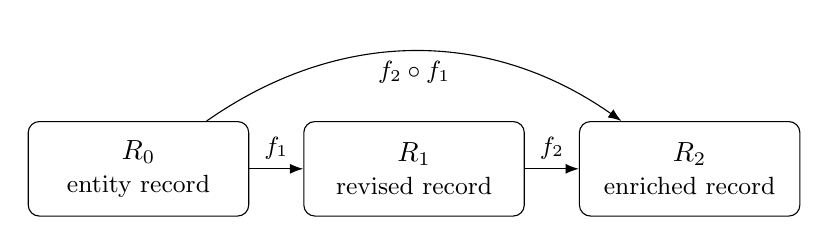
\begin{tikzpicture}[
      node distance=3.5cm,
      state/.style={rectangle,rounded corners,draw,minimum width=2.8cm,minimum height=1.2cm,align=center},
      >=Latex
    ]
    \node[state] (R0) {$R_0$\\{\small entity record}};
    \node[state,right of=R0] (R1) {$R_1$\\{\small revised record}};
    \node[state,right of=R1] (R2) {$R_2$\\{\small enriched record}};

    \draw[->] (R0) -- node[above]{\small $f_1$} (R1);
    \draw[->] (R1) -- node[above]{\small $f_2$} (R2);
    \draw[->, bend left=35]
    (R0) to node[below]{\small $f_2 \circ f_1$} (R2);
  \end{tikzpicture}

  \caption{Morphisms in $\mathbf{CEP}$ as provenance-preserving transformations.
    Each arrow corresponds to a valid record evolution that preserves schema
    validity, revision monotonicity, and canonical identity.}
  \label{fig:cep-morphisms}
\end{figure}

% ------------------------------------------------------------
\subsection*{D.2 Naturality of Attestations}
% ------------------------------------------------------------

Figure~\ref{fig:naturality-attestations} visualizes attestations as a
natural transformation between two envelope functors
$\mathcal{E}, \mathcal{E}' : \mathbf{P} \to \mathbf{E}$.

\begin{figure}[ht]
  \centering
  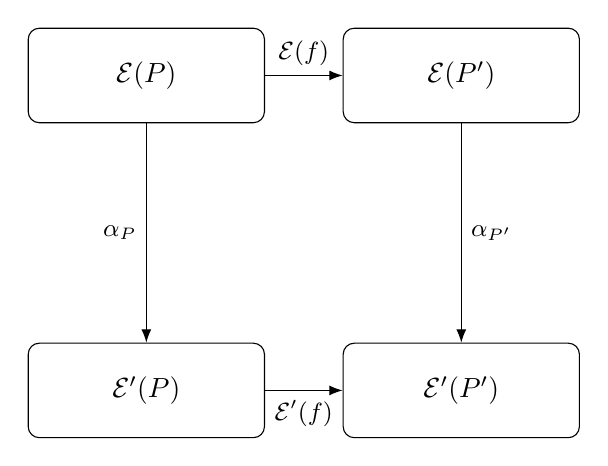
\begin{tikzpicture}[
      node distance=4.0cm,
      obj/.style={rectangle,rounded corners,draw,minimum width=3.0cm,minimum height=1.2cm,align=center},
      >=Latex
    ]
    \node[obj] (EP) {$\mathcal{E}(P)$};
    \node[obj,right of=EP] (EPP) {$\mathcal{E}(P')$};
    \node[obj,below of=EP] (E2P) {$\mathcal{E}'(P)$};
    \node[obj,below of=EPP] (E2PP) {$\mathcal{E}'(P')$};

    \draw[->] (EP) -- node[above]{\small $\mathcal{E}(f)$} (EPP);
    \draw[->] (E2P) -- node[below]{\small $\mathcal{E}'(f)$} (E2PP);
    \draw[->] (EP) -- node[left]{\small $\alpha_P$} (E2P);
    \draw[->] (EPP) -- node[right]{\small $\alpha_{P'}$} (E2PP);
  \end{tikzpicture}
  \caption{Naturality square for attestations.
    The equality
    $\alpha_{P'} \circ \mathcal{E}(f) = \mathcal{E}'(f) \circ \alpha_P$
    expresses that attestation commutes with valid transformations of payloads.}
  \label{fig:naturality-attestations}
\end{figure}

% ------------------------------------------------------------
\subsection*{D.3 Canonicalization Pipeline}
% ------------------------------------------------------------

Figure~\ref{fig:canonicalization-pipeline-appendix} summarizes the canonicalization
pipeline: normalization, assembly, and hashing.

\begin{figure}[ht]
  \centering
  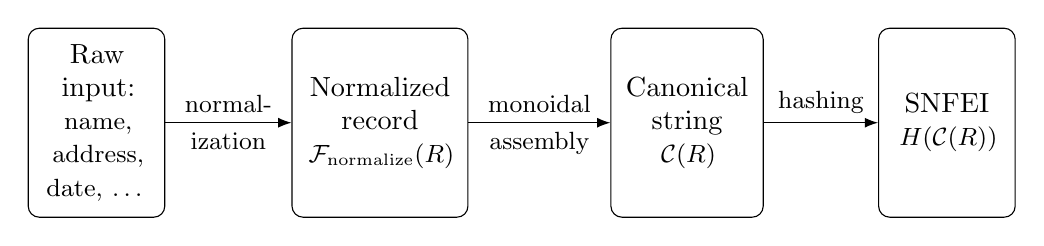
\begin{tikzpicture}[
      stage/.style={
          rectangle,
          rounded corners,
          draw,
          minimum width=1.5cm,
          minimum height=2.4cm,
          align=center
        },
      >=Latex
    ]
    % Explicit positions
    \node[stage, text width=1.5cm] at (0,0)   (raw)   {Raw input:\\{\small name, address, date, \dots}};
    \node[stage, text width=2cm] at (3.6,0) (norm)  {Normalized record\\{\small $\mathcal{F}_{\text{normalize}}(R)$}};
    \node[stage, text width=1.7cm] at (7.5,0)   (canon) {Canonical string\\{\small $\mathcal{C}(R)$}};
    \node[stage, text width=1.5cm] at (10.8,0) (hash) {SNFEI\\{\small $H(\mathcal{C}(R))$}};

    % Arrows from right edge to left edge
    \draw[->] (raw.east)   --
    node[above]{\small normal-}
    node[below]{\small ization}
    (norm.west);
    \draw[->] (norm.east) --
    node[above]{\small monoidal}
    node[below]{\small assembly}
    (canon.west);
    \draw[->] (canon.east) -- node[above]{\small hashing}  (hash.west);
  \end{tikzpicture}
  \caption{The canonicalization pipeline as a composition of a
    normalization functor, a strict monoidal assembly functor, and a
    hashing endofunctor that collapses canonical strings to identifiers.}
  \label{fig:canonicalization-pipeline-appendix}
\end{figure}


% ------------------------------------------------------------
\subsection*{D.4 Jurisdictional Adapters as Oplax Functors}
% ------------------------------------------------------------

Figure~\ref{fig:oplax-adapter-appendix} illustrates the weakened coherence
condition for an oplax functor
$\mathcal{A} : \mathbf{J_{local}} \to \mathbf{J_{global}}$.

\begin{figure}[ht]
  \centering
  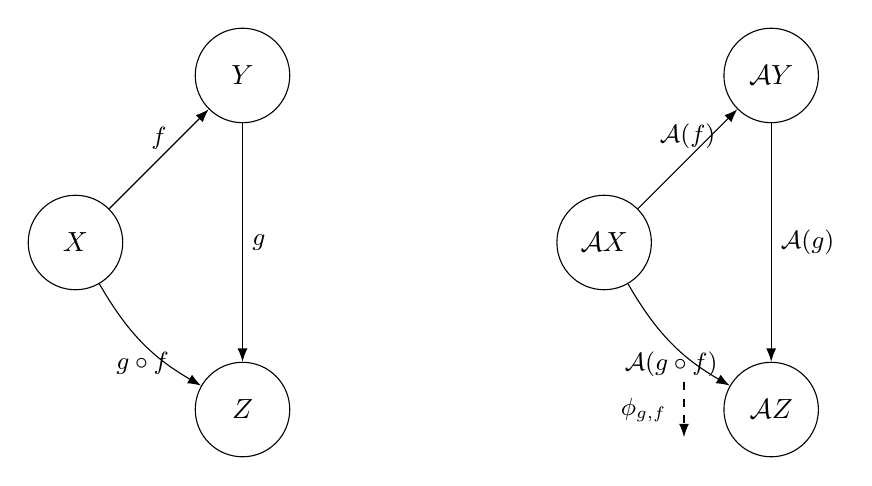
\begin{tikzpicture}[
      node distance=3.0cm,
      obj/.style={circle,draw,minimum size=1.2cm,align=center},
      >=Latex
    ]
    % Local side
    \node[obj] (X) {$X$};
    \node[obj,above right of=X] (Y) {$Y$};
    \node[obj,below right of=X] (Z) {$Z$};

    \draw[->] (X) -- node[above]{\small $f$} (Y);
    \draw[->] (Y) -- node[right]{\small $g$} (Z);
    \draw[->,bend right=15] (X) to node[below]{\small $g \circ f$} (Z);

    % Global side
    \node[obj,right=5.5cm of X] (AX) {$\mathcal{A}X$};
    \node[obj,above right of=AX] (AY) {$\mathcal{A}Y$};
    \node[obj,below right of=AX] (AZ) {$\mathcal{A}Z$};

    \draw[->] (AX) -- node[above]{\small $\mathcal{A}(f)$} (AY);
    \draw[->] (AY) -- node[right]{\small $\mathcal{A}(g)$} (AZ);
    \draw[->,bend right=15] (AX) to node[below]{\small $\mathcal{A}(g \circ f)$} (AZ);

    % Coherence 2-cell: vertical dashed arrow left of AZ
    \draw[->, dashed]
    ($(AZ.west) + (-0.5,0.35)$) -- ($(AZ.west) + (-0.5,-0.35)$)
    node[midway,left,xshift=-0.1cm]{\small $\phi_{g,f}$};

  \end{tikzpicture}
  \caption{Oplax coherence for a jurisdictional adapter
    $\mathcal{A} : \mathbf{J_{local}} \to \mathbf{J_{global}}$.
    The dashed 2-cell $\phi_{g,f}$ witnesses that
    $\mathcal{A}(g \circ f)$ and $\mathcal{A}(g) \circ \mathcal{A}(f)$
    need not coincide strictly, reflecting possible lossy or partial mappings.}
  \label{fig:oplax-adapter-appendix}
\end{figure}

% ------------------------------------------------------------
\subsection*{D.5 Context Tags as a Fibration}
% ------------------------------------------------------------
% Intent: fibers over a base with some functor between them
% Two base objects R and R'
% A base arrow f : R → R'
% Vertical fibers of tags above each
% Solid arrows down to the base (projection)
% Dashed arrows between the fibers (reindexing)
% For a (Grothendieck) fibration
% Given a base arrow  f : R → R'
% standard reindexing is contravariant and we pull back tags along f

Figure~\ref{fig:fibration-ctags} shows the projection
$\pi : \mathbf{CT} \to \mathbf{CEP}$ and the fibers of context tags
above a base record.

\begin{figure}[ht]
  \centering
  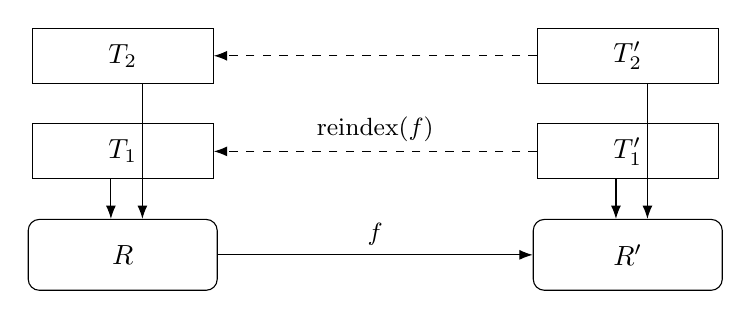
\begin{tikzpicture}[
      node distance=2.4cm,
      base/.style={rectangle,rounded corners,draw,minimum width=2.4cm,minimum height=0.9cm,align=center},
      tag/.style={rectangle,draw,minimum width=2.3cm,minimum height=0.7cm,align=center},
      >=Latex
    ]
    % Base objects
    \node[base] (R) {$R$};
    \node[base,right=4cm of R] (Rp) {$R'$};

    \draw[->] (R) -- node[above]{\small $f$} (Rp);

    % Fiber over R
    \node[tag,above=0.5cm of R] (T1) {$T_1$};
    \node[tag,above=0.5cm of T1] (T2) {$T_2$};

    % Fiber over R'
    \node[tag,above=0.5cm of Rp] (T1p) {$T'_1$};
    \node[tag,above=0.5cm of T1p] (T2p) {$T'_2$};

    % Projections over R
    \draw[->] ($(T1.south) + (-0.15cm,0)$) -- ($(R.north) + (-0.15cm,0)$);
    \draw[->] ($(T2.south) + (0.25cm,0)$)  -- ($(R.north) + (0.25cm,0)$);

    % Projections over R'
    \draw[->] ($(T1p.south) + (-0.15cm,0)$) -- ($(Rp.north) + (-0.15cm,0)$);
    \draw[->] ($(T2p.south) + (0.25cm,0)$)  -- ($(Rp.north) + (0.25cm,0)$);

    % Reindexing along f, fiber over R' -> fiber over R
    \draw[->,dashed] (T1p) -- node[above]{\small $\mathrm{reindex}(f)$} (T1);
    \draw[->,dashed] (T2p) -- (T2);

  \end{tikzpicture}
  \caption{Context tags as a fibration $\pi : \mathbf{CT} \to \mathbf{CEP}$.
    Each base record $R$ has a fiber of permitted tags above it.
    A morphism $f : R \to R'$ induces a reindexing between fibers,
    while the underlying canonical identity remains anchored in the base.}
  \label{fig:fibration-ctags}
\end{figure}
   % Diagrammatic intuition
% !TeX root = 00_cep_semantics.tex
\clearpage
\section*{Appendix E. Glossary for Non-Category Theory Readers}
\addcontentsline{toc}{section}{Appendix E. Glossary for Non-Category Theory Readers}

This appendix provides short, non-technical explanations of the categorical
concepts used in the paper.
The intention is to make the mathematical structure
of CEP more accessible to readers from computer science, data engineering,
public administration, and civic-technology communities.

% ------------------------------------------------------------
\subsection*{E.1 Categories}
A \emph{category} is a mathematical setting that describes:
\begin{itemize}
  \item some \textbf{objects} (things), and
  \item some \textbf{morphisms} (arrows) between them.
\end{itemize}

A category is like a directed graph with rules:
every arrow (morphism) has a source and target,
arrows can be composed,
and each object has an identity arrow that starts from the object, points back to the object, and does nothing.

The latin root \emph{morph} means "form" or "shape",
so a morphism is a way of changing the form of one object into another.

In CEP:
\begin{itemize}
  \item objects = record states,
  \item morphisms = valid record transformations (updates, amendments, joins).
\end{itemize}

Defining CEP as a category formalizes the idea of "things and the allowed changes between them".

% ------------------------------------------------------------
\subsection*{E.2 Functors}
A \emph{functor} is a mapping between categories that preserves structure.
It sends:
\begin{itemize}
  \item each object to another object, and
  \item each morphism to another morphism,
\end{itemize}
in a way that respects composition and identity.

In CEP, a functor often represents a pipeline stage, such as:
\begin{itemize}
  \item wrapping a payload in an envelope,
  \item normalizing noisy text into canonical components,
  \item assembling canonical strings.
\end{itemize}

Functors ensure that if a record evolves legally, its transformed
version evolves legally too.

\emph{Function} and \emph{functor} have the same root and similarities,
but different meanings:
functions map elements within sets,
while functors map objects and morphisms between categories.

% ------------------------------------------------------------
\subsection*{E.3 Natural Transformations}
A \emph{natural transformation} is a structured way of comparing two functors.
If functors are "processing stages", a natural transformation is a
systematic way to convert the output of one stage into the output of another.

In CEP, attestations are modeled as natural transformations:
\begin{itemize}
  \item the envelope functor produces a plain metadata wrapper,
  \item the attested-envelope functor produces a cryptographically validated wrapper.
\end{itemize}

Naturality expresses the idea:
\begin{quote}
  "Whether you process then attest, or attest then process,
  you end up with consistent provenance."
\end{quote}

% ------------------------------------------------------------
\subsection*{E.4 Monoidal Categories}
A \emph{monoidal category} is a category equipped with a notion of
"combining things".

Examples:
\begin{itemize}
  \item strings combine by concatenation,
  \item datasets combine by joining,
  \item workflows combine by sequencing.
\end{itemize}

Canonicalization is the process of converting data into a standard format,
most commonly by selecting a single, preferred output
to represent a piece of content that could have multiple versions.

Canonicalization in CEP is \emph{monoidal} because it combines
individual normalized components into a single canonical string
in a strictly deterministic order.

% ------------------------------------------------------------
\subsection*{E.5 Strict Monoidal Functors}
A \emph{strict monoidal functor} is a functor that preserves the
combination structure \emph{exactly}.

In CEP:
\begin{itemize}
  \item the order of pieces (name, address, date, jurisdiction)
        must always be preserved,
  \item no additional symbols or whitespace are introduced,
  \item the final output is the canonical string fed to the SHA-256 cryptographic hash function.
\end{itemize}

This strictness is what guarantees the stability of the SNFEI identifier.

% ------------------------------------------------------------
\subsection*{E.6 Oplax Functors}
An \emph{oplax functor} preserves structure in a weakened, direction-sensitive way.
The \emph{op} prefix indicates \emph{opposite} directionality and \emph{lax} indicates looseness.
An oplax functor therefore "loosens" structure in a specific direction and
allows "preservation up to a coherence map" rather than strict equality.
A coherence map is a controlled way of relating two structures that are not strictly equal.

It allows:
\begin{itemize}
  \item missing fields,
  \item lossy interpretations,
  \item mappings that preserve meaning but not full structure.
\end{itemize}

Jurisdictional adapters in CEP behave oplaxly because:
\begin{itemize}
  \item local data models may omit fields,
  \item global vocabularies may have stricter typing,
  \item some equivalences hold only "up to" a coherence rule.
\end{itemize}

Oplax behavior models "local autonomy with global convergence".
It means that local jurisdictions can adapt data flexibly
while still ensuring that the global system remains coherent and consistent.

% ------------------------------------------------------------
\subsection*{E.7 Pullbacks (Consistent Joins)}
A \emph{pullback} is the categorical notion of a \emph{consistent join}.

If two data sources both refer to the \emph{same entity or event},
the pullback constructs the most precise version of their agreement.

This formalizes CEP's guarantee that:
\begin{quote}
  Records may be joined only when they assert compatible facts.
\end{quote}

A pullback enables us to formally define the data fusion operation that
combines records from different schemas while preserving:
\begin{itemize}
  \item canonical identity,
  \item vocabulary-governed semantics,
  \item provenance constraints.
\end{itemize}

\emph{Data fusion} refers to the process of integrating multiple data sources
to produce more consistent, accurate, and useful information than that
provided by any individual source.

% ------------------------------------------------------------
\subsection*{E.8 Fibered Categories}
A \emph{fibered category} describes a setting where each object has a
family of additional structures "above it".

CEP is a fibered category.
In CEP:
\begin{itemize}
  \item the base category is $\mathbf{CEP}$,
  \item the fibers contain context tags (CTags).
\end{itemize}

This cleanly separates:
\begin{itemize}
  \item \textbf{identity} (in the base category), and
  \item \textbf{interpretation or annotation} (in the fiber).
\end{itemize}

CTags provide information about a record, without affecting the canonical SNFEI identifier.

% ------------------------------------------------------------
\subsection*{E.9 Universal Properties}
A \emph{universal property} describes an object that is "best" or "most canonical" for a specific purpose.

SNFEI behaves like a universal property construction because:

\begin{itemize}
  \item it is determined by a canonical string,
  \item it is invariant under allowed morphisms,
  \item any other identifier consistent with CEP's invariants must factor uniquely through this construction.
\end{itemize}

This is the mathematical justification enabling us to treat SNFEI
as a stable, verifiable, compositional global identifier.

  % ------------------------------------------------------------
  {\small
    \subsection*{E.10 Summary Table}
    \begin{center}
      \begin{tabular}{p{0.23\linewidth} p{0.35\linewidth} p{0.32\linewidth}}
        \toprule
        \textbf{Concept}        & \textbf{Intuition}       & \textbf{CEP Role}         \\
        \midrule
        Category                & Things, allowed changes  & Record states and updates \\
        Functor                 & Structure-preserving map & Normalization, envelopes  \\
        Natural transformation  & Coherent comparison      & Attestations              \\
        Monoidal category       & Combine things           & Canonical assembly        \\
        Strict monoidal functor & Combine exactly          & SNFEI stability           \\
        Oplax functor           & Weak structure map       & Jurisdiction adapters     \\
        Pullback                & Consistent join          & Merging record fragments  \\
        Fibered category        & Object annotations       & CTags above records       \\
        Universal property      & Optimal construction     & Identifier uniqueness     \\
        \bottomrule
      \end{tabular}
    \end{center}
  }

% ------------------------------------------------------------
\subsection*{E.11 Closing Note}
These notions are not introduced for abstraction's sake;
they express precisely and formally the structural guarantees
CEP requires to support interoperability, trust, and cross-jurisdiction governance.

These mathematical definitions allow the protocol to be:
\begin{itemize}
  \item modular in its design,
  \item formally verifiable in its behavior,
  \item capable of operating consistently even when sources use different schemas, vocabularies, or jurisdictional rules,
  \item and extensible to future domains.
\end{itemize}

By grounding CEP in category theory,
we provide a rigorous foundation for its design principles and operational claims.
   % Glossary of CAE terms (not category theory)

\bibliographystyle{plainnat}
\bibliography{bib_shared}
\end{document}